\section{Adendo}
\label{sec:adendo}

	Caro professor, este adendo apresenta brevemente alguns conteúdos educacionais produzidos no CEPA, por mim ou sob a minha coordenação. Optei por não inserir este material no memorial propriamente dito pois ele requereria explicações que iriam além do propósito dele. Por outro lado, creio que apenas pelo texto seja muito difícil imaginar o que estamos fazendo. Daí este adendo: seu intuito é dar uma ideia do que sejam esses \foreign{softwares} educacionais.
	
	\begin{figure}
		\centering
		\begin{minipage}[b]{0.46\textwidth}
			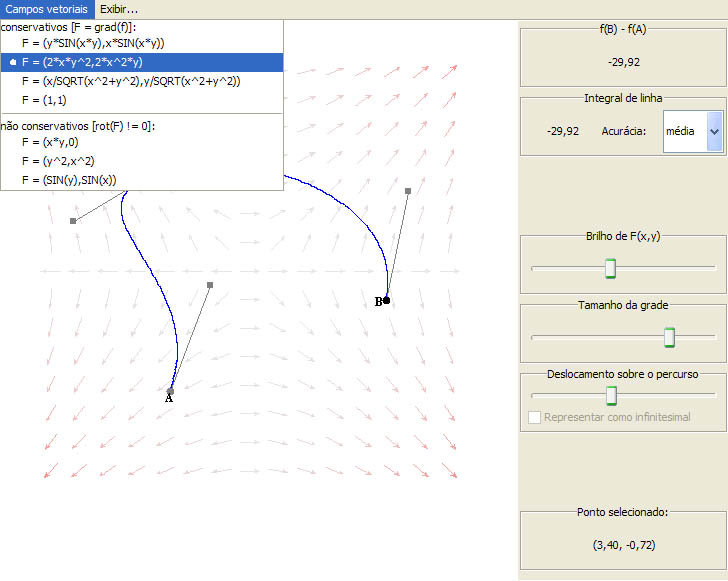
\includegraphics[width=\textwidth]{images/campo-vetorial.jpg}
			\caption{\footnotesize primeiro \foreign{applet} Java desenvolvido para o CEPA, em dezembro de 2007. Este recurso é expositivo, mas permite ao usuário interagir de modo a comparar seus cálculos com aqueles apresentados pelo \foreign{software}.}
			\label{fig:campo}
		\end{minipage}\hfill
		\begin{minipage}[b]{0.46\textwidth}
			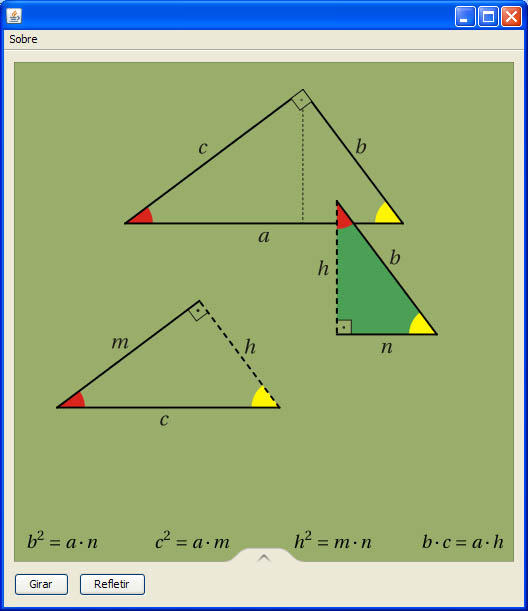
\includegraphics[width=\textwidth]{images/triangulo-retangulo.jpg}
			\caption{\footnotesize \foreign{software} desenvolvido para a proposta de aula interativa do CEPA, em maio de 2009. Este recurso é expositivo e colaborativo, pois foi feito para ser executado em lousas eletrônicas.}
			\label{fig:rel-metr}
		\end{minipage}
	\end{figure}
	
	A figura~\ref{fig:campo} ilustra o primeiro \foreign{applet} Java que desenvolvi quando ingressei no CEPA, em dezembro de 2007. Seu propósito é explorar os conceitos de integral de linha e de campos vetoriais conservativos ($\vec u = -\nabla f$) e não-conservativos. Essencialmente, o \foreign{software} exibe o valor da integral de linha, calculada numericamente.
	
	Inicialmente, o \foreign{software} disponibiliza um campo vetorial (conservativo) e um percurso fáceis de manipular, para que o usuário possa fazer os cálculos por conta própria, tanto da integral de linha quanto de $f(B) - f(A)$, oriundo do teorema fundamental do cálculo. Em seguida, ele é orientado a modificar o percurso, sem mover os pontos $A$ e $B$, e a perceber que a integral não muda (consequência do campo ser conservativo). Diferentemente, quando o usuário escolhe um campo não-conservativo, a integral altera-se com qualquer mudança no percurso. Este recurso está disponível \href{http://cepa.if.usp.br/old/files/simulation/javaapplet/PathIntegralAtContainer.html}{aqui}.
	
	A figura~\ref{fig:rel-metr} ilustra o aplicativo que foi desenvolvido especialmente para a proposta de aula interativa com lousa eletrônica do CEPA, para o projeto Aulas Interativas. Seu intuito é \emph{auxiliar o professor} a deduzir as relações métricas do triângulo-retângulo: o professor arrasta de dentro do triângulo maior (no topo) os dois triângulos-retângulos internos, e pode rotacioná-los e refletí-los convenientemente, de modo que fique evidente a relação de semelhança entre eles. Desta forma, o professor pode deduzir muito facilmente as relações, sem os embaraços da abordagem tradicional. Por exemplo, a relação $c^2 = a \cdot m$ pode ser deduzida observando-se os lados $a$ e $c$ do triângulo superior e os lados $c$ e $m$ daquele à esquerda: por semelhança, $c/m = a/c$, o que resulta na relação métrica.
	
	Pelo que observei nas apresentações desta aula, a simplicidade desta dedução foi o que realmente cativou os professores da Secretaria de Estado da Educação, e creio que tenha contribuido decisivamente para a participação do CEPA no projeto.
	
	\begin{figure}
		\centering
		\begin{minipage}[t]{0.46\textwidth}
			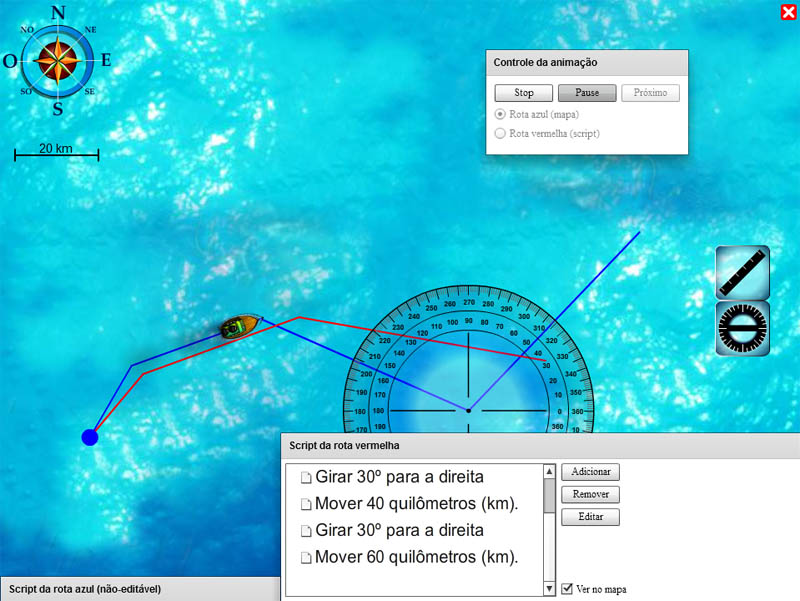
\includegraphics[width=\textwidth]{images/navigation.jpg}
			\caption{\footnotesize recurso desenvolvido para a disciplina de Matemática do 6\textordmasculine\ do Ensino Fundamental (projeto Aulas Interativas). Como o anterior, é expositivo e colaborativo, mas também permite avaliação do aluno, através da comparação entre os trajetos azul e vermelho.}
			\label{fig:nav}
		\end{minipage}\hfill
		\begin{minipage}[t]{0.46\textwidth}
			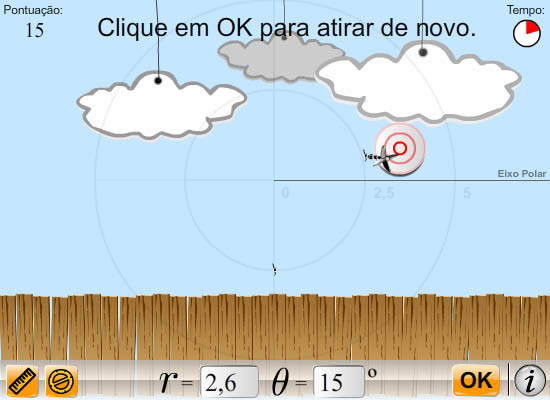
\includegraphics[width=\textwidth]{images/polar.jpg}
			\caption{\footnotesize este \foreign{software} foi desenvolvido para a Univesp, e traz uma abordagem mais próxima dos jogos eletrônicos. Ele também permite avaliação e foi feito para aulas a distância.}
			\label{fig:polar}
		\end{minipage}
	\end{figure}
	
	
	A figura~\ref{fig:nav} representa uma das atividades interativas que produzimos para o projeto Aulas Interativas, para a disciplina de Matemática do 6\textordmasculine\ ano do Ensino Fundamental. O intuito dela é permitir ao professor expor e exercitar, de maneira lúdica, conceitos como pontos cardeais, escala, medidas de ângulo e de distância, e até uma introdução à programação de computadores.
	
	Por exemplo, o professor pode desenhar uma trajetória (azul) arbitrária para o navio e, em seguida, pedir que os alunos representem aquela trajetória em termos de uma sequência de comandos \emph{mover}, \emph{girar} e \emph{repetir}. Isto também é feito no \foreign{software} (na lousa eletrônica), e é representado pelo script na base da imagem. Para executar esta tarefa a contento, os alunos devem utilizar a régua e o transferidor disponibilizados no \foreign{software}, bem como a escala do mapa. E para conferir a resposta, o professor pode habilitar a visualização desse caminho, em vermelho. Alternativamente, o professor pode escrever o script (rota em vermelho) e pedir que os alunos a desenhem, em azul. Observe ainda que o professor pode executar a animação do navio percorrendo a trajetória azul ou a vermelha passo-a-passo, e assim discutir cada instrução dada no script.
	
	Particularmente com relação a este \foreign{software}, outra possibilidade que chamou a atenção dos Professores Coordenadores das Oficinas Pedagógicas foi a possibilidade de ilustrar como é que o computador desenha uma curva: basta colocar uma instrução do tipo \emph{repetir 10 vezes os comandos: mover \unit{10}{\kilo\metre} e girar \unit{10}{\degree}}.
	
	Finalmente, a figura~\ref{fig:polar} ilustra outro recurso, este feito para a Univesp. Seu objetivo é permitir ao usuário \emph{familiarizar-se} com os sistema de coordenadas polar. Ao pressionar o botão \emph{ok} o alvo é aleatoriamente posicionado na tela, e cabe ao usuário acertá-lo com um dardo. Para lançar o dardo o usuário deve informar quais são as coordenadas, $r$ e $\theta$, do alvo. E quanto mais próximas da resposta, mais próximo do alvo o dardo chega e, por conseguinte, mais pontos ele faz. Há uma régua e um transferidor à disposição do usuário (embaixo, à esquerda), de modo que ele pode medir as coordenadas com precisão. No entanto, há um tempo limite para dar a resposta, e quanto mais rápido ele resolve a questão, mais pontos ele faz. Assim, para maximizar sua pontuação o usuário acaba concluindo, depois de algumas tentativas e erros, que é melhor \emph{estimar} a resposta. E deste modo espera-se que ele se familizarize com as coordenadas polares. Este recurso está disponível em \href{http://midia.atp.usp.br/atividades-interativas/AI-0001/}{aqui}.
	